% ------------------------------------------------------------------------------
% Este fichero es parte de la plantilla LaTeX para la realización de Proyectos
% Final de Grado, protegido bajo los términos de la licencia GFDL.
% Para más información, la licencia completa viene incluida en el
% fichero fdl-1.3.tex

% Copyright (C) 2012 SPI-FM. Universidad de Cádiz
% ------------------------------------------------------------------------------

Este capítulo trata sobre todos los aspectos relacionados con la implementación
del sistema en código, haciendo uso de un determinado entorno tecnológico.

\section{Entorno tecnológico}
En esta sección se indica el marco tecnológico utilizado para la construcción
del sistema, como son:
\begin{itemize}
    \item Entorno de desarrollo (IDE).
    \item Lenguaje de programación, bibliotecas y frameworks de desarrollo
          empleados.
    \item Herramientas de ayuda a la construcción y despliegue.
    \item Control de versiones y repositorio de componentes.
\end{itemize}

El lenguaje de programación utilizado para la elaboración del proyecto ha sido
Python, usándose multitud de bibliotecas de todas las que ofrece el lenguaje,
pero en especial, se ha hecho uso de la biblioteca \textit{rdflib}, la cual ha
permitido tanto el parseo de fichero rdf, como la generación del rdf para la
exportación de datos, en diferentes formatos.

Dentro del lenguaje Python, se ha utilizado el framework \textit{Django}, ya que
el proyecto básicamente consiste en el desarrollo de un plugin para dicho
framework. Además del framework Django, también se ha hecho uso de otros
frameworks, los cuales facilitasen tanto la escritura de estilos CSS como de
código JavaScript. Estos frameworks auxiliares utilizados son \textit{jQuery}
\cite{jQuery} y \textit{Bootstrap} \cite{Bootstrap}.

Tanto en la importación de vocabularios para la aplicación como en la
publicación de los datos, ha sido necesario utilizar formatos específicos, como
son el caso de \textit{RDF/XML}, \textit{RDF/Ntriples}, \textit{RDF/Turtle},
\textit{RDFa} o \textit{Microdata}. Además, en la importación de los datos de
los vocabularios, ha sido necesario utilizar el lenguaje de consultas
\textit{SPARQL}, que permite realizar consultas sobre conjuntos de datos
definidos en ficheros RDF. También se ha hecho uso del software D2Rq, que ofrece
al usuario a partir del esquema de la base de datos, múltiples utilidades para
la publicación de sus datos en internet.

Como IDE de desarrollo, se ha utilizado un editor de texto simple, en este caso
gEdit, con plugins para programación, y el resaltado de código python. A su vez,
también se han utilizado herramientas proporcionadas por la comunidad Python
para la depuración del código, tales como \textit{iPython} y \textit{ipdb}.

Para el despliegue del proyecto se ha utilizado el servidor de pruebas que
ofrece el framework Django, y el servidor \textit{Apache} junto con el
intérprete de apache para código Python \textit{mod\_wsgi}.

Por último, para el alojamiento del código fuente y demás ficheros que componen
el proyecto, se ha hecho uso del sistema de control de versiones
\textit{subversion}, integrado el mismo con la aplicación \textit{Redmine} para
la gestión de tareas y asignaciones de tiempo.

\section{Código fuente}
La organización del código fuente del proyecto, se ha llevado a cabo siguiendo
las indicaciones del propio framework Django para la estructura de sus
aplicaciones, de tal forma que en directorio raíz del proyecto cabría destacar
los siguientes subdirectorios y ficheros:
\begin{itemize}
    \item \textbf{forms:} en este directorio se encuentran alojados todos los
        formularios Django que se utilizan dentro de la aplicación. A su vez,
        este directorio está compuesto por el directorio modelforms, que
        contiene todos los formularios basados en modelos de Django.
    \item \textbf{decorators:} en este directorio se encuentran implementado el
        decorador utilizado en las vistas, para comprobar que el usuario que
        intenta acceder a ellas, se encuentra logueado y tiene permisos de
        superusuario.
    \item \textbf{locale:} en este directorio se encuentran las traducciones de
        la aplicación a los diferentes idiomas que soporta la misma.
        Inicialmente está soportado los idiomas inglés y español.
    \item \textbf{management:} este directorio contiene a su vez el directorio
        commands, el cual contiene todos los comandos desarrollados, a fin de
        que puedan ser ejecutados desde el manage.py de Django desde una
        terminal.
    \item \textbf{models:} este directorio contiene todos los modelos que
        componen a la aplicación Django. Contiene un fichero por cada uno de los
        modelos de la aplicación.
    \item \textbf{parsing:} este directorio no es común a todo proyecto Django,
        pero se encarga de agrupar todas las clases y métodos necesarios para el
        parseo y carga de ontologías en formato RDF.
    \item \textbf{static:} este directorio compuesto a su vez por un
        subdirectorio cuyo nombre es el mismo de la aplicación, se encarga de
        almacenar todos los elementos estáticos de la aplicación, ya sean
        imágenes, estilos, código JavaScript, etc.
    \item \textbf{templates:} este directorio compuesto también a su vez por un
        subdirectorio con el mismo nombre de la aplicación, se encarga de
        almacenar todas las plantillas del proyecto django.
    \item \textbf{templatetags:} este directorio contiene todos los template
        tags desarrollados que pueden ser usados en las plantillas django. Se
        divide en dos ficheros, easydata\_microdata y easydata\_rdfa, y cada
        uno de ellos contienen los template tags necesarios para exportar la
        información en formato microdata y rdfa respectivamente.
    \item \textbf{views:} este directorio contiene todos los ficheros python con
        las vistas que se usarán en la aplicación. Existen varios ficheros, y se
        encargan de agrupar las vistas por funcionalidades comunes.
    \item \textbf{urls.py:} contiene todas las asociaciones de urls con las
        distintas vistas de la aplicación.
    \item \textbf{utils.py:} contiene multitud de funciones auxiliares que se
        utilizan tanto para el mapeo de modelos, como para la exportación de los
        datos en distintos formatos.
\end{itemize}

\subsection{Internacionalización y localización}

A la hora de desarrollar el software EasyData/Django se ha tenido en cuenta que
el mismo pueda ofrecer su contenido en diferentes idiomas en función de los
diferentes usuarios.

Para preparar el software para que este pueda ser traducido a diferentes idiomas
(internacionalización) se han seguido las recomendaciones de Django y se han
hecho uso de las herramientas que proporciona, tanto para la traducción de
cadenas en el código Python como para la traducción de las plantillas. De igual
forma, se ofrecen las traducciones de la aplicación (localización) en los
idiomas inglés y español.

\section{Calidad de código}

Para asegurar la calidad del código fuente y por consiguiente, su fácil
mantenibilidad, además de estructurar la aplicación tal y como recomienda Django,
se ha seguido la guía de estilos para escribir código Python llamada PEP8. La
guía de estilos PEP8 proporciona una serie de convenciones para la codificación
en Python. De esta forma, además de proporcionarme una forma de trabajo y de
escribir un código claro, nos aseguramos en cierta medida, que el código será
fácilmente entendible por cualquier programador que esté acostumbrado a utilizar
esta guía de estilos. A parte del
\href{http://www.python.org/dev/peps/pep-0008/}{manual PEP8} que se encuentra
publicado en la web oficial de Python, existe una herramienta para diferentes
sistemas operativos, con el mismo nombre que la guía de estilos, que comprueba
directamente si nuestro código cumple con las especificaciones de pep8.

Además de la guía de estilos PEP8, también se ha utilizado la herramienta PyLint
que proporciona una métrica que permite obtener una idea de en qué medida el
código de la aplicación es de calidad. Para obtener dicha métrica se basa en
diferentes como puede ser:
\begin{itemize}
    \item Cantidad de comentarios de código (ni poco comentado ni
        sobrecomentado), que no existan elementos como clases, funciones o
        modulos sin comentar.
    \item Que se cumplan patrones de diseño como el patron DRY (Don't repeat
        yourself), de tal forma que no existan abundantes sentencias de código
        repetidas.
    \item Que el proyecto se encuentre correctamente estructurado.
    \item Cumplimiento de convenciones en la escritura del códgio fuente, como
        en el nombre de variables, clases, interlineado, etc\ldots
    \item Que no existan errores en el código.
\end{itemize}

Una vez ejecutada la prueba de calidad de código con PyLint, se ha obtenido una
puntuacion de 9,3 sobre 10 para el código de la aplicación, haciendo uso de un
fichero de configuración de PyLint específico para proyectos Django. Además solo
existe un 1,345\% de líneas duplicadas (89 líneas) de entre mas de 5000 líneas
de código que ha abarcado la aplicación. El resultado es el que se puede
apreciar en la figura \ref{fig:pylint}.

La finalidad de realizar estas pruebas de código, además de que el código
escrito cumpla con un mínimo de calidad, sirve a título personal para la
adquisición de buenas prácticas a la hora de programar, las cuales se puedan
poner en práctica en futuros proyectos.

\begin{figure}[H]
    \begin{center}
        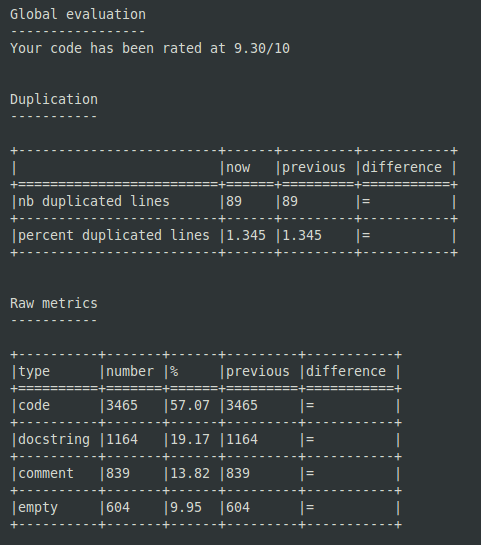
\includegraphics[width=0.6\textwidth]{pruebas/pylint.png}
    \end{center}
    \caption{Resultado de pruebas de validación de PyLint}
    \label{fig:pylint}
\end{figure}
